\documentclass[12pt]{article}
\usepackage[utf8]{inputenc}
\usepackage{amsmath,amsfonts}
\usepackage{graphicx}
\usepackage{hyperref}
\usepackage{float}
\usepackage{geometry}
\usepackage{wrapfig}
\geometry{margin=1in}

\title{\textbf{Simulating Simon's Algorithm Under Noise with Qiskit}}
\author{Emmanuel Valdovinos Cota \\ PHYS 160: Intro. to Quantum Computing \\ University of California, Riverside}
\date{\today}

\begin{document}

\maketitle

\begin{abstract}
We implement and simulate Simon’s Algorithm using Qiskit to investigate its performance in both ideal and noisy environments. By applying noise models through IBM’s quantum runtime, we evaluate the resilience and practical limitations of this foundational quantum algorithm.
\end{abstract}

\section*{Introduction}

Quantum computing promises to solve certain computational problems exponentially faster than classical approaches. This potential is most strikingly demonstrated through quantum algorithms, which exploit superposition and entanglement to achieve dramatic speedups. Among the earliest and most foundational of these is Simon's Algorithm, which was the first to show an exponential separation between quantum and classical computing in the query complexity model.

Simon's problem is a promise problem involving a hidden binary string $s$ such that for a given black-box function $f$, we have $f(x) = f(x \oplus s)$ for all inputs $x$. The classical solution to this problem requires an exponential number of queries, while the quantum solution, with Simon's Algorithm, solves it with a polynomial number of queries, leveraging the ability of quantum circuits to extract global properties of $f$ more efficiently.

This algorithm directly influenced the development of Shor’s factoring algorithm, which also exploits hidden periodicity, and thus plays a key historical role in demonstrating the power of quantum computation.

In this paper, we implement and simulate Simon’s Algorithm using IBM’s Qiskit platform. We first analyze the algorithm’s behavior under ideal, noiseless conditions. We then introduce realistic noise models to study how quantum decoherence and gate errors impact the success rate of the algorithm. By simulating the algorithm under both conditions, we aim to better understand its strengths and fragilities, and to provide insight into the challenges of achieving quantum advantage on near-term devices.

\section*{Background}

Simon’s Problem asks us to determine a hidden binary string $s \in \{0,1\}^n$ given a function $f: \{0,1\}^n \rightarrow \{0,1\}^m$ such that $f(x) = f(y)$ if and only if $x \oplus y = s$ for some fixed, unknown $s$. The function is guaranteed to be either one-to-one (if $s = 0^n$) or two-to-one, with each output value corresponding to exactly two inputs differing by $s$.

Classically, solving this problem requires $\mathcal{O}(2^{n/2})$ queries in the worst case, because it involves identifying two distinct inputs with the same output. However, Simon’s Algorithm solves it with only $\mathcal{O}(n)$ queries on a quantum computer.

The quantum approach leverages superposition and interference to reveal information about $s$. The algorithm prepares a uniform superposition over all possible $n$-bit inputs, applies the function $f$ as an oracle, and then measures part of the system. After applying a Hadamard transform to the remaining register, the resulting measurements produce binary strings $y$ that satisfy $y \cdot s = 0 \pmod{2}$. After collecting roughly $n$ such linearly independent equations, the hidden string $s$ can be recovered by solving the system of equations over $\text{GF}(2)$ (Galois Field of order 2).

Simon’s Algorithm is not only important for its speedup, but because it laid conceptual groundwork for later breakthroughs such as Shor’s Algorithm. Both exploit hidden structures that classical computers find hard to extract, but which quantum systems can detect through interference.

\section*{Implementation}

In this section, we describe how Simon’s Algorithm was implemented using Qiskit and IBM’s Quantum Runtime platform. The implementation includes both an ideal (noiseless) version and a noisy version using Qiskit's built-in noise models.

\subsubsection*{Oracle Construction}
To implement the required two-to-one function, the oracle circuit applies CNOT gates based on the bits of the hidden string $s$. For each index $i$ where $s_i = 1$, a CNOT gate maps the input qubit $q_i$ to the output qubit $q_{n+i}$. This ensures that $f(x) = f(x \oplus s)$ as required by Simon's Problem.

\subsubsection*{Quantum Circuit Design}

The resulting measurement outputs are binary strings $y$ satisfying the constraint $y \cdot s = 0 \pmod{2}$. After collecting enough such strings, the hidden value $s$ can be recovered using classical linear algebra.

\begin{figure}[H]
    \centering
    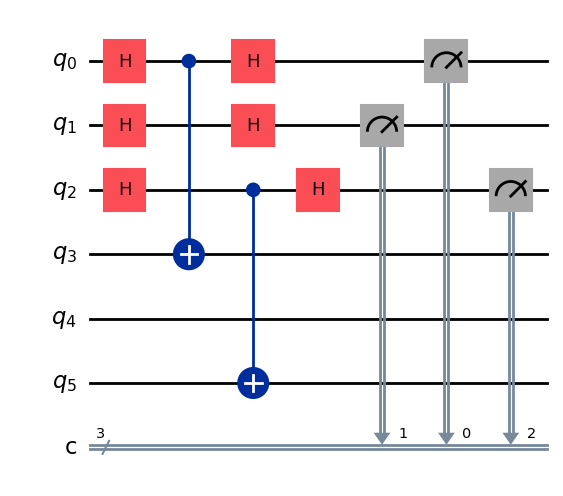
\includegraphics[width=0.50\textwidth]{simon_circuit.png}
    \label{fig:simon_circuit}
\end{figure}

With the oracle defined, we construct the full Simon's Algorithm circuit. The circuit begins by applying Hadamard gates to each input qubit to place them in a uniform superposition. After querying the oracle, another round of Hadamard gates is applied to the input register to extract information about the hidden string $s$.

\subsubsection*{Results Under Ideal and Noisy Conditions}

\begin{figure}[H]
    \centering
    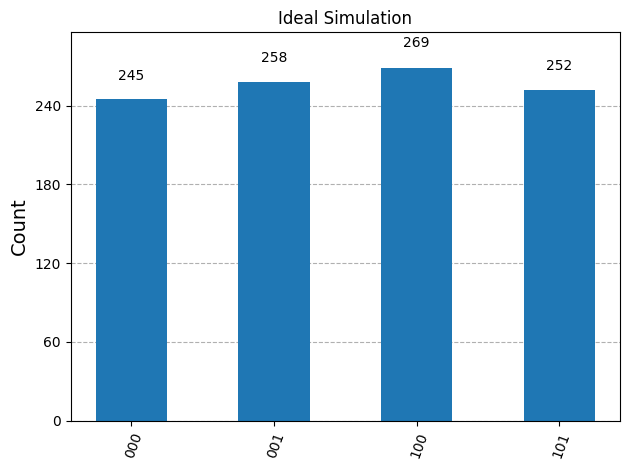
\includegraphics[width=0.45\textwidth]{ideal.png}
    \hfill
    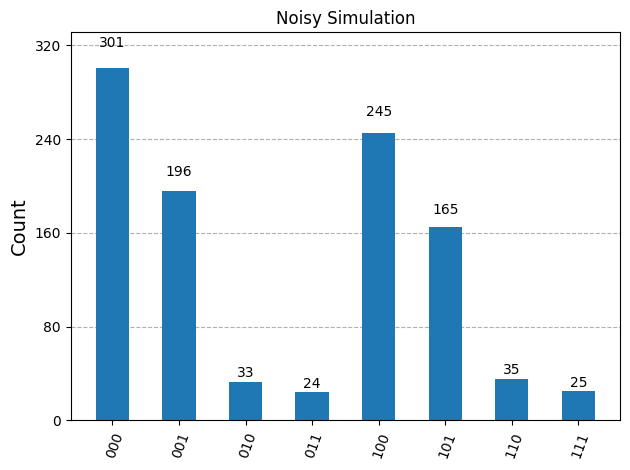
\includegraphics[width=0.45\textwidth]{noisy.png}
    \label{fig:histograms}
\end{figure}

Under ideal conditions, Simon’s Algorithm yields a small set of valid output strings that satisfy the relation $y \cdot s = 0 \pmod{2}$. These are consistent with the expected quantum behavior of the algorithm and enable the reconstruction of the hidden string $s$ through classical post-processing.

When simulated with noise, however, the results deviate. A wider range of output strings appears, including many that do not satisfy the constraint. This is due to gate and readout errors introduced by the noise model. The increase in spurious results illustrates the algorithm’s sensitivity to noise and underscores the need for quantum error correction or noise mitigation in practical implementations.

\section*{References}
\begin{itemize}
  \item Young, R. \textit{An Undergraduate Course on Quantum Computing}, Chapter 12, pp. 105–108.
  \item Mulligan, M. \textit{Graduate Quantum Mechanics Lecture Notes}, Chapter 18, pp. 295–297.
  \item AWS Quantum Blog. “Simon’s Algorithm.” \url{https://aws.amazon.com/blogs/quantum-computing/simons-algorithm/}
  \item Sadhukhan, T. “Simon’s Algorithm.” \textit{ResearchGate}, 2024. \url{https://www.researchgate.net/publication/389826581_Simon's_Algorithm}
  \item IBM Qiskit Documentation. “Install Qiskit.” \url{https://quantum.cloud.ibm.com/docs/en/guides/install-qiskit}
  \item Coding Tech. “Simon’s Algorithm Explained.” YouTube Playlist. \url{https://www.youtube.com/watch?v=93-zLTppFZw}
  \item Matplotlib. “Interactive Figures in Jupyter with ipympl.” \url{https://matplotlib.org/ipympl/}
  \item Qiskit Tutorials. “Advanced Circuit Visualization.” GitHub. \url{https://github.com/Qiskit/qiskit-tutorials/blob/master/tutorials/circuits_advanced/03_advanced_circuit_visualization.ipynb}
\end{itemize}

\section*{Note}
This project was developed as part of PHYS 160: Introduction to Quantum Computing at the University of California, Riverside. The complete implementation, simulation notebooks, and figures are available at: 

\url{https://github.com/Emmanuel-va1d/phys160-simulating-simons-algorithm.git}

\end{document}
